\section{CHIRP Sequence Configuration}

\label{sec:chirp-theory}

To enable effective ego-motion estimation, the radar must be configured with a suitable chirp profile that balances range and velocity resolution.
This is achieved through the configuration of Frequency-Modulated Continuous Wave (FMCW) chirps, which define how the radar sweeps frequencies over time to capture environmental information.

In millimeter-wave FMCW radar systems such as the IWR6843, a chirp refers to a signal whose frequency increases (or decreases) linearly over a defined bandwidth $B$ during a fixed duration $T_c$.
When this signal reflects off a target and returns to the radar, the delay between transmitted and received signals encodes range information.
The Doppler shift between multiple received chirps in a frame encodes relative velocity.  
As seen in Figure~\ref{fig:radarWavePropagation}, the reflected wave varies in phase and frequency depending on object motion.


\begin{figure}[!htbp]
    \centering
    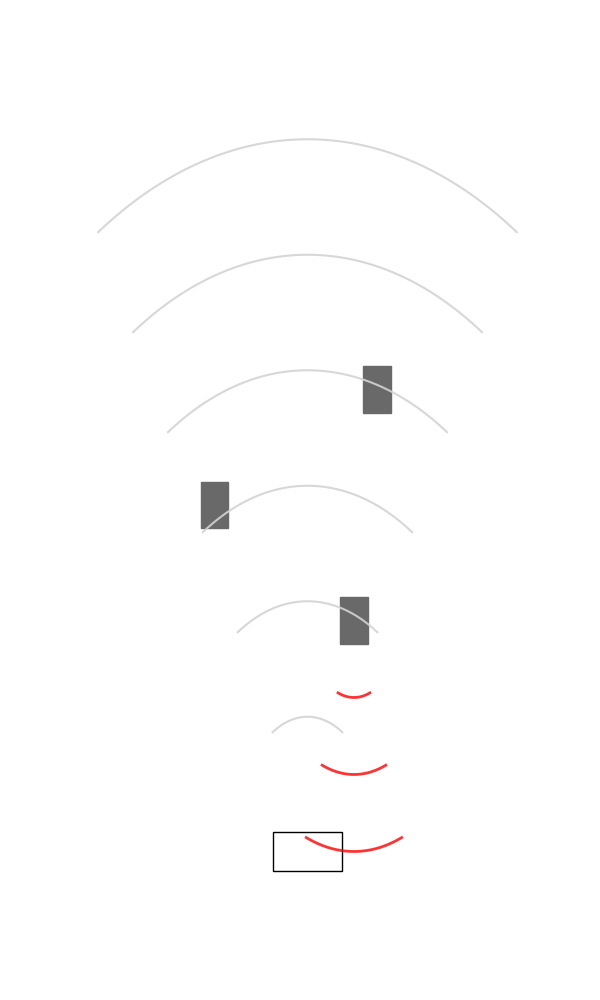
\includegraphics[width=0.5\linewidth]{images/radarWave.png}
    \caption{Radar 60-64GHz radio wave reflection.}
    \label{fig:radarWavePropagation}
\end{figure}

Each chirp is defined by the following core parameters:
\begin{itemize}
    \item Start frequency $f_0$
    \item Frequency slope $S$
    \item Chirp duration $T_c$
    \item Idle time between chirps $T_{idle}$
    \item Sampling rate $f_s$
    \item Bandwidth $B = S \cdot T_c$
\end{itemize}

\hfill

From these parameters, the radar sensing capabilities are derived as follows:

\begin{itemize}
    \item \textbf{Range resolution:} 
    \[
        \Delta R = \frac{c}{2B}
    \]
    where $c$ is the speed of light and $B$ is the chirp bandwidth.

    \item \textbf{Maximum unambiguous range:} 
    \[
        R_{max} = \frac{c f_s}{2S}
    \]
    where $f_s$ is the ADC sampling rate and $S$ is the frequency slope.

    \item \textbf{Velocity resolution:} 
    \[
        \Delta v = \frac{\lambda}{2 N_c T_c}
    \]
    where $\lambda$ is the wavelength, $N_c$ is the number of chirps per frame, and $T_c$ is the chirp duration.

    \item \textbf{Maximum unambiguous velocity:} 
    \[
        v_{max} = \frac{\lambda}{4 T_c}
    \]
    assuming uniform chirp spacing.
\end{itemize}

These equations clearly show that both range and velocity resolution depend directly on the chirp design.

\vspace{1em}
\newpage

\subsection{Chirp Design Strategies and Trade-offs}
\label{sec:chirp-strategies}

Radar applications differ in their emphasis on range vs velocity accuracy.
Odometry requires both.
We now examine key chirp configuration strategies and discuss their trade-offs.
\vspace{1em}

\subsubsection*{(1) Full-Bandwidth Chirp (Single 4~GHz Sweep)}

A single chirp sweeping across the entire 4~GHz available bandwidth provides the finest possible range resolution.
This is ideal for tasks requiring precise spatial localization of static objects.

\textbf{Trade-offs:}
\begin{itemize}
    \item \textbf{Pros:} Excellent range resolution ($\Delta R$ minimized).
    \item \textbf{Cons:} High ADC sampling rates required. Limits maximum measurable range ($R_{max}$). Increases noise sensitivity. Not ideal for multi-radar systems due to potential mutual interference.
\end{itemize}

\begin{figure}[!htbp]
    \centering
    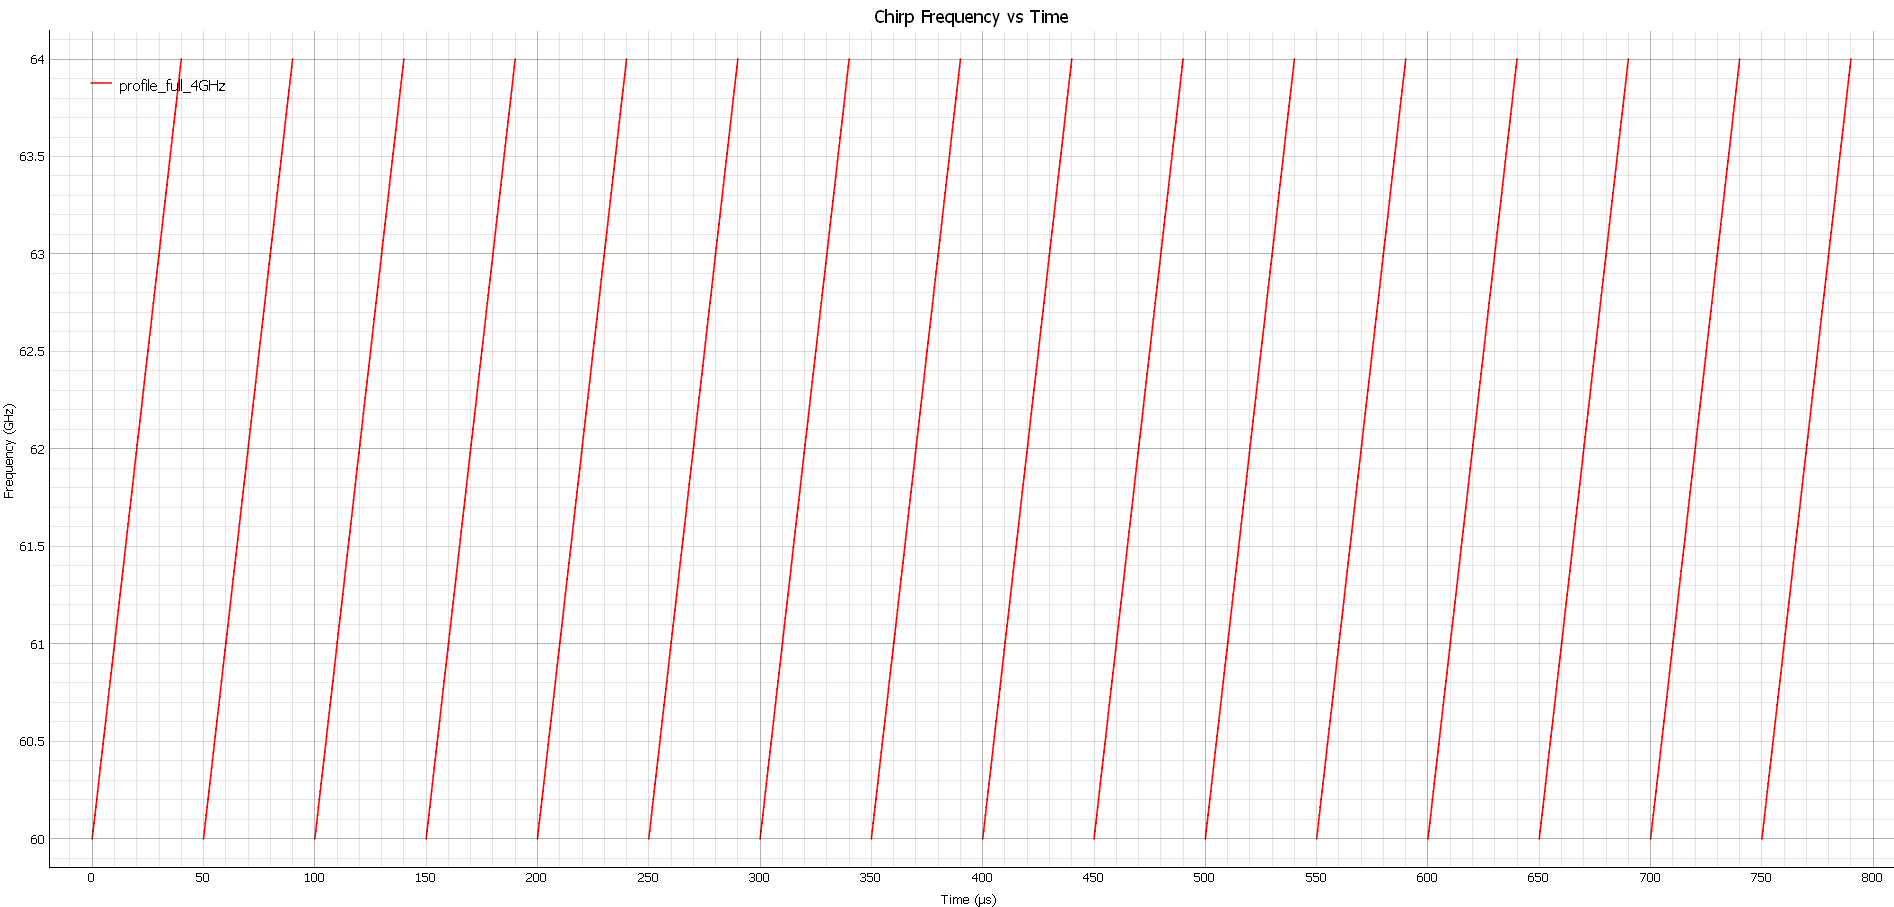
\includegraphics[width=1.0\linewidth]{images/profile_full_4GHz.png}
    \caption{Single 4~GHz chirp.}
    \label{fig:profile4GHz}
\end{figure}

{\small
\textit{Conclusion:} Best for high-resolution mapping in single-device systems.
May suffer in multi-radar setups due to wide spectral overlap.
}

\vspace{1em}

\subsubsection*{(2) Divided-Band Chirps (Multiple Shorter Sweeps)}

An alternative is to split the full 4~GHz bandwidth into multiple chirps with reduced individual sweep widths (e.g., 2~GHz).
Each chirp provides moderate resolution.

\textbf{Trade-offs:}
\begin{itemize}
    \item \textbf{Pros:} Reduced ADC load. Allows frequency diversity across chirps.
    \item \textbf{Cons:} Each individual chirp has worse $\Delta R$ than full sweep. However, averaging multiple bands improves robustness.
\end{itemize}

\begin{figure}[!htbp]
    \centering
    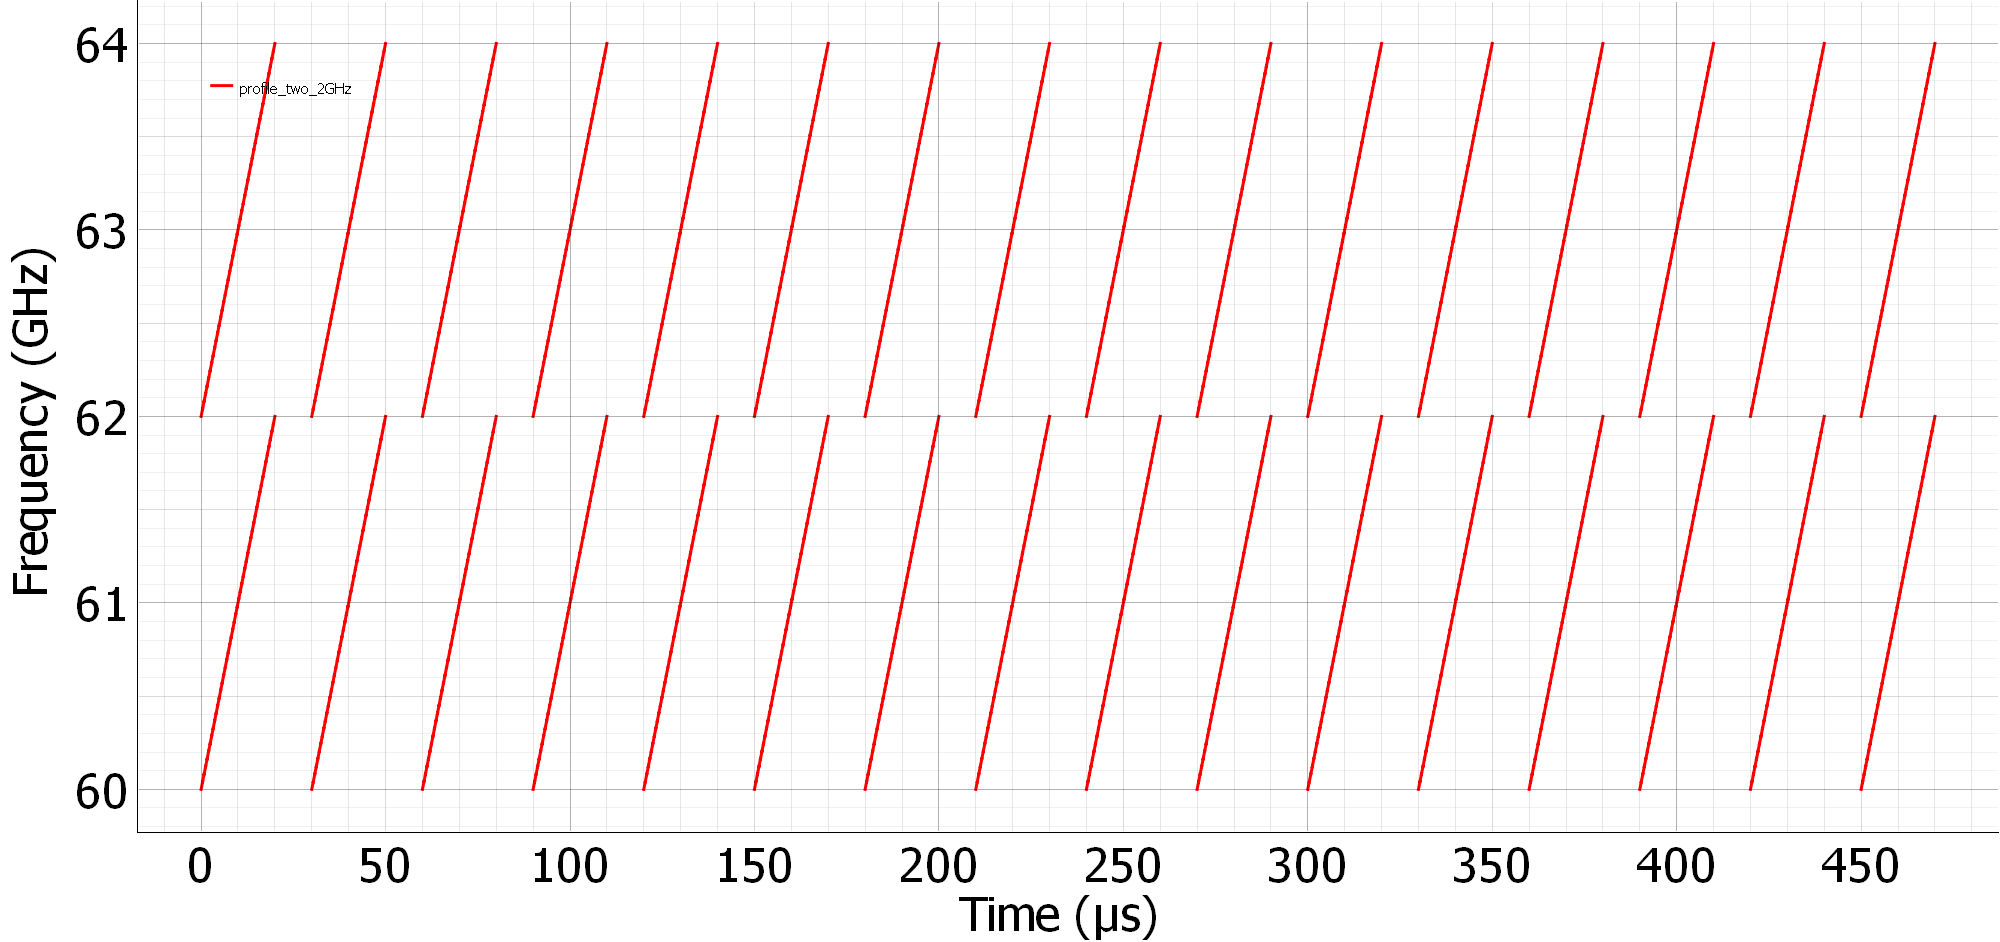
\includegraphics[width=1.0\linewidth]{images/profile_two_2GHz.png}
    \caption{Two 2~GHz chirps in the same frame.}
    \label{fig:profile2GHz}
\end{figure}

{\small
\textit{Conclusion:} Balanced design.
Useful in scenarios requiring robustness against channel noise or radar interference.
Also reduces overlap when multiple radars are active.
}

\vspace{1em}

\subsubsection*{(3) Mixed Chirp Strategy (Full-Band + Narrow-Band Chirps)}

Combining different chirp types in a single frame can provide both high range and velocity resolution.
For example, use one full-band chirp for precise range, followed by multiple narrow-band chirps for velocity estimation.

\textbf{Trade-offs:}
\begin{itemize}
    \item \textbf{Pros:} Leverages benefits of both strategies. Improves multi-parameter resolution without overwhelming hardware.
    \item \textbf{Cons:} Increases configuration complexity. Requires advanced processing and careful interleaving.
\end{itemize}

\begin{figure}[!htbp]
    \centering
    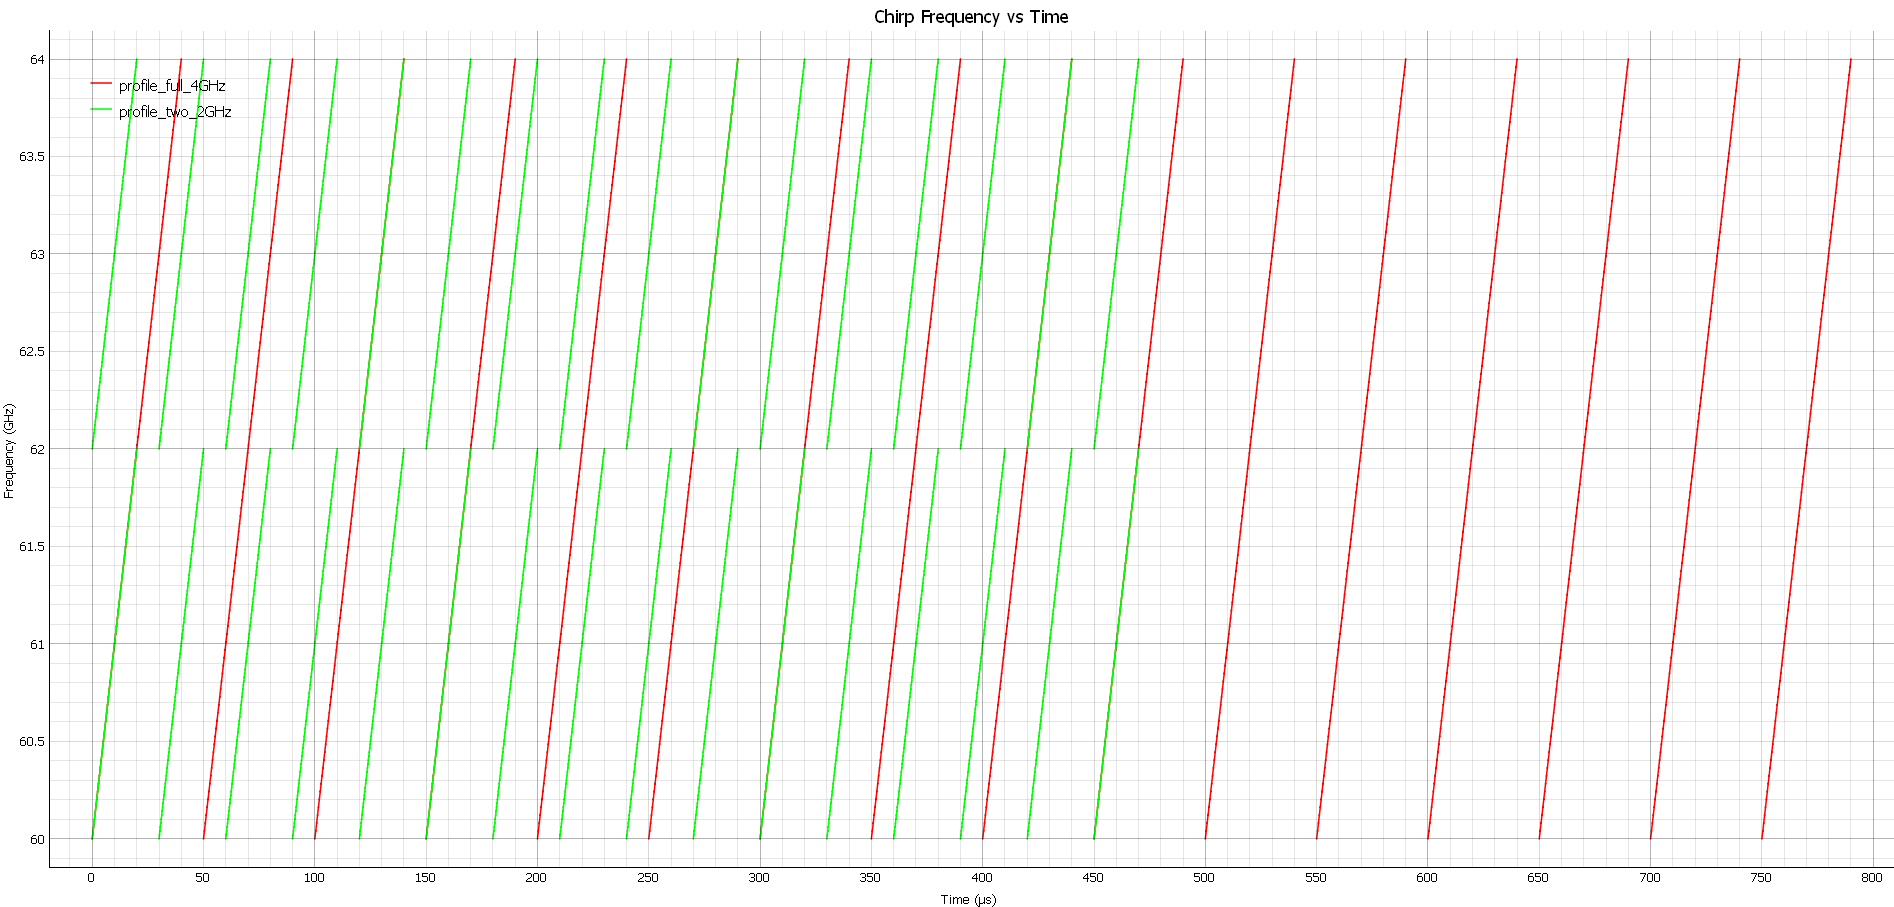
\includegraphics[width=1.0\linewidth]{images/profile_full_4GHz_2GHz.png}
    \caption{Overlay of single 4~GHz chirp and two 2~GHz chirps.}
    \label{fig:profile2And4GHz}
\end{figure}

{\small
\textit{Conclusion:} Best suited for ego-motion and odometry applications.
Can support multi-device environments with careful planning.
}

\begin{table}[h]
    \centering
    \caption{Comparison of Chirp Configuration Strategies}
    \label{tab:chirp_comparison}
    \resizebox{\columnwidth}{!}{%
    \begin{tabular}{|p{3.5cm}|p{3.2cm}|p{3.5cm}|p{3.8cm}|}
        \hline
        \textbf{Chirp Strategy} & \textbf{Range Resolution} & \textbf{Velocity Resolution} & \textbf{Best Use Case} \\
        \hline
        Full-Bandwidth Chirp (4 GHz) &
        High (Fine $\Delta R$) &
        Moderate (Few chirps/frame) &
        Precise mapping in single-radar setups; spatial accuracy prioritized \\
        \hline
        Divided-Band Chirps (e.g., 2×2 GHz) &
        Moderate (per chirp), improved via averaging &
        Moderate to High (more chirps/frame possible) &
        Robust odometry in noisy or multi-radar environments \\
        \hline
        Mixed Chirp Strategy (Full + Narrow) &
        High (from full chirp), plus enhanced Doppler &
        High (from multiple narrow chirps) &
        Ego-motion estimation; combines benefits of both range and Doppler precision \\
        \hline
    \end{tabular}%
    }
\end{table}

\vspace{1em}

The table above summarizes the key performance characteristics and use cases for each chirp configuration strategy.

The Full-Bandwidth Chirp maximizes spatial resolution, making it ideal for scenarios where high-fidelity mapping of nearby static objects is required—such as indoor SLAM or obstacle-rich environments. 
However, its wide spectral footprint and high ADC demand make it less suitable in systems where multiple radar devices operate simultaneously, as mutual interference becomes likely.
The Divided-Band Chirp approach offers a middle ground.
By allocating portions of the spectrum to separate chirps, it reduces system load and provides flexibility in processing. 
While individual chirps have lower range resolution, combining information across them improves detection stability. This strategy excels in distributed radar systems, such as in collaborative or multi-node sensor networks, where frequency coordination helps reduce ghost targets and interference.
Finally, the Mixed Chirp Strategy integrates the strengths of both previous approaches. 
A full-band chirp ensures accurate spatial anchoring, while narrow-band chirps provide temporal and Doppler refinement. 
This makes it the most adaptive option for applications like ego-motion estimation, where both precise localization and motion cues are critical. 
Its complexity, however, demands a more advanced signal processing pipeline and careful calibration to ensure synchronization between chirps.

In multi-radar environments, especially in close proximity (e.g., autonomous fleets or dual-radar vehicles), selecting chirp strategies that reduce spectral overlap is essential. Techniques like time-division multiplexing, slope diversity, and chirp staggering become critical tools to mitigate false detections and interference.

\vspace{1em}

\subsection{Chirp Configuration for Multi-Radar Systems}
\label{sec:chirp-multiradar}

When deploying multiple radar devices (e.g., front-left, front-right), interference becomes a significant challenge.
Simultaneous transmission using overlapping chirp frequencies can lead to ghost detections, false targets, and degraded signal-to-noise ratio. 
This due to the radio waves that are transmitter can cause collitions between each other creating this "ghost detections".
There are some strategies that can be employed to avoid this phenomenom.

\textbf{Recommended strategies:}
\begin{itemize}
    \item Use \textbf{non-overlapping frequency ranges} per device (e.g., 60–62~GHz on left, 62–64~GHz on right).
    \item Apply \textbf{interleaved chirps} in time: stagger chirps across sensors.
    \item Utilize \textbf{different slope values}: reduces likelihood of constructive interference.
    \item Match chirp \textbf{idle times} to ensure orthogonality.
\end{itemize}

These methods are essential to avoid ghost detections and preserve spatial coherence across sensors.

\vspace{1em}

{\small
\textit{Conclusion:} Chirp configuration in multi-radar environments requires trade-offs between resolution and isolation.  
Design must ensure orthogonality to avoid mutual interference.
}

\vspace{1em}

The configuration of chirps in FMCW radar defines its core capabilities in range and velocity estimation.
Depending on the target application — whether precision mapping, ego-motion tracking, or multi-device deployment — the choice of chirp bandwidth, duration, slope, and sequencing must be carefully made.

The following considerations are essential:
\begin{itemize}
    \item Use wide-band chirps when range precision is critical.
    \item Use many chirps with long frame durations when velocity resolution is prioritized.
    \item Use divided-band or mixed strategies in multi-radar systems to balance robustness and prevent interference.
\end{itemize}

Careful design enables robust radar odometry, reliable environment mapping, and scalable multi-radar systems.
